% Options for packages loaded elsewhere
\PassOptionsToPackage{unicode}{hyperref}
\PassOptionsToPackage{hyphens}{url}
%
\documentclass[
  man,floatsintext]{apa6}
\usepackage{amsmath,amssymb}
\usepackage{lmodern}
\usepackage{iftex}
\ifPDFTeX
  \usepackage[T1]{fontenc}
  \usepackage[utf8]{inputenc}
  \usepackage{textcomp} % provide euro and other symbols
\else % if luatex or xetex
  \usepackage{unicode-math}
  \defaultfontfeatures{Scale=MatchLowercase}
  \defaultfontfeatures[\rmfamily]{Ligatures=TeX,Scale=1}
\fi
% Use upquote if available, for straight quotes in verbatim environments
\IfFileExists{upquote.sty}{\usepackage{upquote}}{}
\IfFileExists{microtype.sty}{% use microtype if available
  \usepackage[]{microtype}
  \UseMicrotypeSet[protrusion]{basicmath} % disable protrusion for tt fonts
}{}
\makeatletter
\@ifundefined{KOMAClassName}{% if non-KOMA class
  \IfFileExists{parskip.sty}{%
    \usepackage{parskip}
  }{% else
    \setlength{\parindent}{0pt}
    \setlength{\parskip}{6pt plus 2pt minus 1pt}}
}{% if KOMA class
  \KOMAoptions{parskip=half}}
\makeatother
\usepackage{xcolor}
\usepackage{graphicx}
\makeatletter
\def\maxwidth{\ifdim\Gin@nat@width>\linewidth\linewidth\else\Gin@nat@width\fi}
\def\maxheight{\ifdim\Gin@nat@height>\textheight\textheight\else\Gin@nat@height\fi}
\makeatother
% Scale images if necessary, so that they will not overflow the page
% margins by default, and it is still possible to overwrite the defaults
% using explicit options in \includegraphics[width, height, ...]{}
\setkeys{Gin}{width=\maxwidth,height=\maxheight,keepaspectratio}
% Set default figure placement to htbp
\makeatletter
\def\fps@figure{htbp}
\makeatother
\setlength{\emergencystretch}{3em} % prevent overfull lines
\providecommand{\tightlist}{%
  \setlength{\itemsep}{0pt}\setlength{\parskip}{0pt}}
\setcounter{secnumdepth}{-\maxdimen} % remove section numbering
% Make \paragraph and \subparagraph free-standing
\ifx\paragraph\undefined\else
  \let\oldparagraph\paragraph
  \renewcommand{\paragraph}[1]{\oldparagraph{#1}\mbox{}}
\fi
\ifx\subparagraph\undefined\else
  \let\oldsubparagraph\subparagraph
  \renewcommand{\subparagraph}[1]{\oldsubparagraph{#1}\mbox{}}
\fi
\newlength{\cslhangindent}
\setlength{\cslhangindent}{1.5em}
\newlength{\csllabelwidth}
\setlength{\csllabelwidth}{3em}
\newlength{\cslentryspacingunit} % times entry-spacing
\setlength{\cslentryspacingunit}{\parskip}
\newenvironment{CSLReferences}[2] % #1 hanging-ident, #2 entry spacing
 {% don't indent paragraphs
  \setlength{\parindent}{0pt}
  % turn on hanging indent if param 1 is 1
  \ifodd #1
  \let\oldpar\par
  \def\par{\hangindent=\cslhangindent\oldpar}
  \fi
  % set entry spacing
  \setlength{\parskip}{#2\cslentryspacingunit}
 }%
 {}
\usepackage{calc}
\newcommand{\CSLBlock}[1]{#1\hfill\break}
\newcommand{\CSLLeftMargin}[1]{\parbox[t]{\csllabelwidth}{#1}}
\newcommand{\CSLRightInline}[1]{\parbox[t]{\linewidth - \csllabelwidth}{#1}\break}
\newcommand{\CSLIndent}[1]{\hspace{\cslhangindent}#1}
\ifLuaTeX
\usepackage[bidi=basic]{babel}
\else
\usepackage[bidi=default]{babel}
\fi
\babelprovide[main,import]{english}
% get rid of language-specific shorthands (see #6817):
\let\LanguageShortHands\languageshorthands
\def\languageshorthands#1{}
\usepackage{tcolorbox}
\usepackage{caption}
\usepackage{setspace}
\usepackage{relsize}
\usepackage[document,bottom]{ragged2e}
\captionsetup[figure]{labelformat=empty}
\captionsetup[table]{labelformat=empty}
\raggedbottom
% Manuscript styling
\usepackage{upgreek}
\captionsetup{font=singlespacing,justification=justified}

% Table formatting
\usepackage{longtable}
\usepackage{lscape}
% \usepackage[counterclockwise]{rotating}   % Landscape page setup for large tables
\usepackage{multirow}		% Table styling
\usepackage{tabularx}		% Control Column width
\usepackage[flushleft]{threeparttable}	% Allows for three part tables with a specified notes section
\usepackage{threeparttablex}            % Lets threeparttable work with longtable

% Create new environments so endfloat can handle them
% \newenvironment{ltable}
%   {\begin{landscape}\centering\begin{threeparttable}}
%   {\end{threeparttable}\end{landscape}}
\newenvironment{lltable}{\begin{landscape}\centering\begin{ThreePartTable}}{\end{ThreePartTable}\end{landscape}}

% Enables adjusting longtable caption width to table width
% Solution found at http://golatex.de/longtable-mit-caption-so-breit-wie-die-tabelle-t15767.html
\makeatletter
\newcommand\LastLTentrywidth{1em}
\newlength\longtablewidth
\setlength{\longtablewidth}{1in}
\newcommand{\getlongtablewidth}{\begingroup \ifcsname LT@\roman{LT@tables}\endcsname \global\longtablewidth=0pt \renewcommand{\LT@entry}[2]{\global\advance\longtablewidth by ##2\relax\gdef\LastLTentrywidth{##2}}\@nameuse{LT@\roman{LT@tables}} \fi \endgroup}

% \setlength{\parindent}{0.5in}
% \setlength{\parskip}{0pt plus 0pt minus 0pt}

% Overwrite redefinition of paragraph and subparagraph by the default LaTeX template
% See https://github.com/crsh/papaja/issues/292
\makeatletter
\renewcommand{\paragraph}{\@startsection{paragraph}{4}{\parindent}%
  {0\baselineskip \@plus 0.2ex \@minus 0.2ex}%
  {-1em}%
  {\normalfont\normalsize\bfseries\itshape\typesectitle}}

\renewcommand{\subparagraph}[1]{\@startsection{subparagraph}{5}{1em}%
  {0\baselineskip \@plus 0.2ex \@minus 0.2ex}%
  {-\z@\relax}%
  {\normalfont\normalsize\itshape\hspace{\parindent}{#1}\textit{\addperi}}{\relax}}
\makeatother

% \usepackage{etoolbox}
\makeatletter
\patchcmd{\HyOrg@maketitle}
  {\section{\normalfont\normalsize\abstractname}}
  {\section*{\normalfont\normalsize\abstractname}}
  {}{\typeout{Failed to patch abstract.}}
\patchcmd{\HyOrg@maketitle}
  {\section{\protect\normalfont{\@title}}}
  {\section*{\protect\normalfont{\@title}}}
  {}{\typeout{Failed to patch title.}}
\makeatother

\usepackage{xpatch}
\makeatletter
\xapptocmd\appendix
  {\xapptocmd\section
    {\addcontentsline{toc}{section}{\appendixname\ifoneappendix\else~\theappendix\fi\\: #1}}
    {}{\InnerPatchFailed}%
  }
{}{\PatchFailed}
\keywords{Blind data analysis; preregistration; ALSPAC; meta-research; open science; Explore and Confirm Analysis Workflow (ECAW)\newline\indent Word count: 4020}
\usepackage{lineno}

\linenumbers
\usepackage{csquotes}
\ifLuaTeX
  \usepackage{selnolig}  % disable illegal ligatures
\fi
\IfFileExists{bookmark.sty}{\usepackage{bookmark}}{\usepackage{hyperref}}
\IfFileExists{xurl.sty}{\usepackage{xurl}}{} % add URL line breaks if available
\urlstyle{same} % disable monospaced font for URLs
\hypersetup{
  pdftitle={Reducing bias in secondary data analysis via an Explore and Confirm Analysis Workflow (ECAW): A proposal and survey of observational researchers},
  pdfauthor={Robert T. Thibault1,2, Marton Kovacs3,4, Tom E. Hardwicke5, Alexandra Sarafoglou6, John P. A. Ioannidis1,7, \& Marcus R. Munafò2,8},
  pdflang={en-EN},
  pdfkeywords={Blind data analysis; preregistration; ALSPAC; meta-research; open science; Explore and Confirm Analysis Workflow (ECAW)},
  hidelinks,
  pdfcreator={LaTeX via pandoc}}

\title{Reducing bias in secondary data analysis via an Explore and Confirm Analysis Workflow (ECAW): A proposal and survey of observational researchers}
\author{Robert T. Thibault\textsuperscript{1,2}, Marton Kovacs\textsuperscript{3,4}, Tom E. Hardwicke\textsuperscript{5}, Alexandra Sarafoglou\textsuperscript{6}, John P. A. Ioannidis\textsuperscript{1,7}, \& Marcus R. Munafò\textsuperscript{2,8}}
\date{}


\shorttitle{Explore and Confirm Analysis Workflow}

\authornote{

Correspondence concerning this article should be addressed to Robert T. Thibault. E-mail: \href{mailto:robert.thibault@stanford.edu}{\nolinkurl{robert.thibault@stanford.edu}}

}

\affiliation{\vspace{0.5cm}\textsuperscript{1} Meta-Research Innovation Center at Stanford (METRICS), Stanford University.\\\textsuperscript{2} School of Psychological Science, University of Bristol.\\\textsuperscript{3} Doctoral School of Psychology, ELTE Eotvos Lorand University, Budapest, Hungary\\\textsuperscript{4} Institute of Psychology, ELTE Eotvos Lorand University, Budapest, Hungary\\\textsuperscript{5} Melbourne School of Psychological Sciences, University of Melbourne.\\\textsuperscript{6} Department of Psychology, University of Amsterdam.\\\textsuperscript{7} Meta-Research Innovation Center Berlin (METRIC-B), QUEST Center for Transforming Biomedical Research, Berlin Institute of Health, Charité -- Universitätsmedizin Berlin.\\\textsuperscript{8} MRC Integrative Epidemiology Unit at the University of Bristol.}

\abstract{%
\justifying\textbf{Background.} Although preregistration can reduce researcher bias and increase transparency in primary research settings, it is less applicable to secondary data analysis. An alternative method that affords additional protection from researcher bias, which cannot be gained from conventional forms of preregistration alone, is an Explore and Confirm Analysis Workflow (ECAW). In this workflow, a data management organization initially provides access to only a subset of their dataset to researchers who request it. The researchers then prepare an analysis script based on the subset of data, upload the analysis script to a registry, and then receive access to the full dataset. ECAWs aim to achieve similar goals as preregistration, but make access to the full dataset contingent on compliance. The present survey aimed to garner information from the research community where ECAWs could be applied---employing the Avon Longitudinal Study of Parents and Children (ALSPAC) as a case example. \hfill \break \hfill \break \textbf{Methods.} We emailed a web-based survey to researchers who had previously applied for access to ALSPAC's transgenerational observational dataset.\hfill \break \hfill \break \textbf{Results}. We received 107 responses, for a 10\% response rate. The results suggest that---at least among our sample of respondents---ECAWs hold the potential to serve their intended purpose and appear relatively acceptable. For example, only 10\% of respondents disagreed that ALSPAC should run a study on ECAWs (versus 55\% who agreed). However, as many as 25\% of respondents agreed that they would be less willing to use ALSPAC data if they were required to use an ECAW (versus 44\% who disagreed).\hfill \break \hfill \break \textbf{Conclusion.} Our data and findings provide information for organizations and individuals interested in implementing ECAWs and related interventions. \hfill \break \hfill \break \textbf{Preregistration:} \url{https://osf.io/g2fw5} Deviations from the preregistration are outlined in Supplementary Material A.
}



\begin{document}
\maketitle

\justifying

\hypertarget{introduction}{%
\section{Introduction}\label{introduction}}

Many published research findings are non-reproducible and potentially false or misleading (Camerer et al., 2016; Collaboration, 2015; Errington et al., 2021; Ioannidis, 2005, 2008). These shortcomings may stem from a combination of researcher bias, publication bias, selective reporting of results, incomplete reporting of methods, and other questionable research practices. These issues can lead to research waste, and ineffective or even harmful healthcare and policy interventions (e.g., see Prasad and Cifu (2019)).

Some research disciplines have adopted standards to address these issues. For example, researchers conducting clinical trials regularly register outcome measures before enrolling participants, and they keep both participants and experimenters blind regarding group assignment. In cases where datasets already exist, however, researchers cannot easily adopt these practices. Researchers performing secondary data analyses generally have access to complete datasets without any blinding imposed on them. This may lead to exploration of diverse analyses and selective reporting based on the nature of the results.

\hypertarget{preregistration-in-the-context-of-secondary-data-analyses}{%
\subsection{Preregistration in the context of secondary data analyses}\label{preregistration-in-the-context-of-secondary-data-analyses}}

Increasing the uptake and effectiveness of preregistration for secondary data analyses may require a different approach than it does for clinical trials. For example, the analytical space for secondary data analyses (e.g., of a longitudinal cohort dataset) is more vast than the analytical space for most clinical trials. Thus, the clinical trial standard of registering outcome measures, but no analysis plan, remains insufficient. Moreover, preregistration of secondary data analyses remains uncommon, and unlike for clinical trials (where the dataset doesn't yet exist), there is no guarantee that researchers performing secondary data analyses haven't accessed the dataset. To extend the benefits of preregistration to secondary data analyses, we propose a workflow that necessitates the preregistration of an executable analysis script before researchers can access the full dataset.

\hypertarget{explore-and-confirm-analysis-workflow-ecaw}{%
\subsection{Explore and Confirm Analysis Workflow (ECAW)}\label{explore-and-confirm-analysis-workflow-ecaw}}

In this intervention we propose, a data management organization that controls access to a preexisting data set would first provide access to only a subset of the data a researcher requests. After the researcher prepares an analysis script based on the subset of data and uploads it to a registry---where it will be openly accessible and permanent (e.g., to the Open Science Framework Registry)---the data management organization then provides access to the full dataset (e.g., via a secure data environment) and the researcher can proceed as they wish. The exact implementation (e.g., whether the data management organization runs quality checks on the analysis scripts) would depend on the preferences of the data management organization and the research community using their dataset (see Box 1 for an hypothetical example).

We call this process an Explore and Confirm Analysis Workflow (ECAW). Researchers may use the subset of data to generate hypotheses and/or to simply ensure that their intended analysis runs properly. ECAWs may increase the uptake of preregistration and provide assurance that the analyses were developed before the researchers observed the full dataset. Moreover, whereas conventional preregistrations often leave many degrees of freedom regarding exactly how the data will be analyzed (e.g., Bakker et al. (2020)), ECAWs provide an executable analysis script. Researchers may also find ECAWs more agreeable than conventional preregistration because they allow for exploration. ECAWs would not fully solve publication bias, but could make it easier to detect because the registered analysis script would serve as a form of preregistration.

In short, ECAWs give researchers access to enough data to develop an informed analysis, but without compromising the confirmatory nature of a final analysis on the complete dataset.

\begin{tcolorbox}
{\fontsize{9pt}{9pt}\selectfont\textbf{Box 1. A hypothetical example of an ECAW in practice.}}

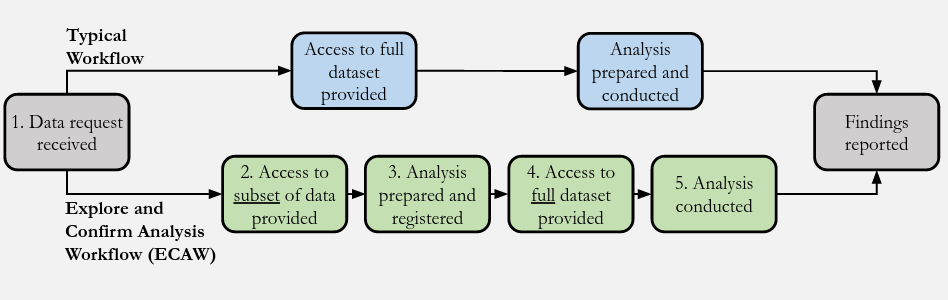
\includegraphics[width=1\textwidth]{./ecaw_workflow.png}
{\fontsize{9pt}{9pt}\selectfont
The overarching framework for ECAWs is depicted above. Within this framework, data management organizations would need to pre-specify several details for each step. Below, we provide a hypothetical example for illustrative purposes. The exact implementation of ECAWs would depend on the preferences of each data management organization and the community who uses their dataset.

\begin{enumerate}
  \item A research team submits to a data management organization (i) a paragraph describing the analyses they want to run, and (ii) a list of the variables they want to analyze.
  \item The data management organization provides the research team with access to a subset of the data. For example, if the research team requests data for 15 variables collected from 10,000 participants, the data management organization will provide access to all 15 variables from a random subset of participants—say 1000.
  \item The research team prepares an analysis script written in a common programming language (e.g., R or Stata) using the subset of data. They register this analysis script, the output from the script, and the paragraph they sent to the data management organization in Step 1, to www.osf.io/registries as an ‘Open-Ended Registration’. The researchers are free to run as many analyses as they would like on the subset of data. However, they should only register the analysis script they plan to use on the complete dataset.
  \item The data management organization performs a basic quality check. They ensure that (i) the analysis script, the script output, and the paragraph are registered, and (ii) the output contains a clear number of itemized results (e.g., as clinicaltrials.gov does for outcome measures). If the quality check fails, the data management organization asks the researchers to update their registration until it passes. The research team is then given access to a dataset with all the variables requested for all participants.
  \item The researchers can proceed as they wish. They can run the registered analysis script on the complete dataset, make adjustments to the analysis if desired, or not proceed at all. The data management organization does not perform any additional check on what analyses were run. Regardless of what the research team decides, a permanent version of the planned analysis is available on the OSF Registry.
\end{enumerate}
}
\end{tcolorbox}

\pagebreak

\hypertarget{examples-of-ecaw-like-workflows}{%
\subsection{Examples of ECAW-like workflows}\label{examples-of-ecaw-like-workflows}}

One study probed the benefits and drawbacks of a workflow similar to ECAWs, but they provided a synthetic dataset rather than a data subset (Sarafoglou, Hoogeveen, and Wagenmakers (2023)). The researchers recruited 120 teams to analyze a single observational dataset and had half the teams preregister a written analysis plan and the other half prepare an analysis plan by drafting an analysis script based on a dataset with shuffled data for the variables of interest (i.e., the analysts were effectively blinded). Based on self-reports from the participants, the researchers found that two workflows were comparable in terms of effort and that teams using blinded data analysis made fewer deviations from their analysis plan.

Some disciplines, such as particle physics, implement blind data analyses regularly (Klein and Roodman (2005); MacCoun and Perlmutter (2015)). A version of the ECAW workflow has also been successfully implemented by eight teams performing secondary data analysis on a dataset managed by the Psychological Science Accelerator group (Forscher et al. (2020)) and is currently being used for Registered Reports based on a large psychology dataset (Schmidt et al. (2023)).

In medicine and clinical epidemiology, a similar workflow is implemented by the software platform OpenSAFELY (www.opensafely.org). This platform provides a dataset of simulated health records from which researchers can develop an analysis script. When ready, a researcher submits their analysis script which is automatically logged and made public in GitHub. The analysis then runs in a Trusted Research Environment (TRE) on data which is stored in the data centers where patients' records already reside (i.e., the data is not copied or moved). This workflow keeps individual health records hidden while also documenting all analyses run on the real data.

\hypertarget{study-objectives}{%
\subsection{Study objectives}\label{study-objectives}}

Here, we present a descriptive and exploratory survey study. We had no hypotheses, but we did have two specific objectives. (1) To gain insights on the opinions and practices of researchers who already use preexisting observational datasets, in regards to the trustworthiness and reproducibility of research. (2) To use these insights to inform future research---including a potential trial of ECAWs with the Avon Longitudinal Study of Parents and Children (ALSPAC)---on how data management organizations can encourage rigorous and reproducible research practices.

\hypertarget{methods}{%
\section{Methods}\label{methods}}

\hypertarget{participants}{%
\subsection{Participants}\label{participants}}

We sent an email to invite researchers on the mailing list for the UK-based Avon Longitudinal Study of Parents and Children (ALSPAC) to participate in an online survey (see Supplementary Material B). We partnered with ALSPAC because they manage an oft-requested dataset and expressed interest in studying ways to ensure the research stemming from their dataset is rigorous. ALSPAC is ``a transgenerational prospective observational study investigating influences on health and development across the life course. It considers multiple genetic, epigenetic, biological, psychological, social and other environmental exposures in relation to a similarly diverse range of health, social and developmental outcomes.'' (Boyd et al., 2013; Fraser et al., 2013). Thus, our invitation reached researchers that use observational data across the health and social sciences. The survey was open from 10 Oct 2022 to 1 Nov 2022. We sent two reminder emails, exactly one week and two weeks after the original email invitation. The mailing list comprises researchers whose email addresses were present on a proposal to access the ALSPAC dataset and included 1148 email addresses.

\hypertarget{survey}{%
\subsection{Survey}\label{survey}}

The survey contained 6 blocks and is available at \url{https://osf.io/5h7gb}. We developed the survey with feedback from the Principal Investigator and Executive Director of ALSPAC (Nicholas Timpson and Kate Northstone). We aimed to include as few questions as possible (to encourage a high response rate) while still garnering substantive information on whether ECAWs are relevant and acceptable to ALSPAC users.

Block 1 assessed the extent to which respondents believe that observational research using preexisting data is trustworthy and reproducible (2 questions). Block 2 asked respondents how often they use practices related to transparency and reducing researcher bias, including preregistration, blinded data analysis, and sharing analysis scripts (5 questions). Between Block 2 and Block 3, the survey described ECAWs. Block 3 assessed the extent to which respondents believe that ECAWs would make observational research using preexisting data more trustworthy and reproducible (2 questions). Block 4 directly asked respondents whether ALSPAC should run a study on ECAWs and whether they would participate (5 questions). Block 5 contained open-ended questions about the perceived benefits and drawbacks of ECAWs, reservations about ECAWs, whether additional incentives might be needed to use ECAW, and suggestions for other research practices or policies that data management organizations could implement to improve research quality (3 questions). Block 6 asked participants how concerned they are about research quality, how many relevant studies they have published, what software they use for data analysis, and for any additional comments (4 questions). All rating-scale questions contained the response option \emph{``I don't understand the question''}. The questions presented in Figure 3 also contained the response option \emph{``Unsure''}.

\hypertarget{analyses}{%
\subsection{Analyses}\label{analyses}}

We present the results for closed-ended questions as prevalence rates or counts in Figures 1-3 and Supplementary Material C. When reporting percentages, we collapse together all positive responses on the rating scales (e.g., \emph{``strongly agree''} and \emph{``somewhat agree''}) as well as all negative responses. The total number of responses differ among questions due to the missing values and responses of \emph{``I don't understand the question''} and \emph{``Unsure''}. We narratively synthesize the responses to the open-ended questions in Table 1 (i.e., we provide a non-systematic qualitative summary).

\hypertarget{results}{%
\section{Results}\label{results}}

\hypertarget{survey-completion}{%
\subsection{Survey completion}\label{survey-completion}}

Of 1148 emails sent, 1094 went through and 54 bounced. The survey was completed 103 times and partially completed 20 times, leading to a response rate of 9\% for complete surveys and 11\% for at least partially complete surveys.\footnote[1]{The ALSPAC mailing list has been maintained as a record of collaborators for many years and is constantly added to. The ALSPAC team only removes email addresses from their mailing list if someone explicitly requests this action. Thus, their list likely includes several email addresses that are no longer monitored. For example, we received one email reply stating that the recipient hasn’t been active in research for 30 years. It is also possible that some researchers have multiple email addresses on the mailing list (e.g., because they moved institutions). These two factors may have deflated the response rate.} The median time to complete the survey was 7.4 minutes (IQR: 4.6 to 13.1). This manuscript presents the results for complete surveys. Supplementary Material D presents the results with partially complete surveys included.

\hypertarget{participants-1}{%
\subsection{Participants}\label{participants-1}}

Respondents had published a median of 10 (IQR 2 to 26) studies using preexisting observational data (Supplementary Figure C1). They reported using the following programming languages or software packages: R (n = 65), Stata (n = 48), SPSS (n = 17), SAS (n = 15), Python (n = 6), Mplus (n = 3), Bash (n = 2), MATLAB (n = 1), Nextflow (n = 1), and plink2 (n = 1) (Supplementary Table C1)\footnote[2]{Participants could select multiple responses to this survey question.}. 62\% (62/100) of participants reported being more concerned with research trustworthiness, bias, rigour, and reproducibility compared to what they think of as a typical research who uses preexisting observational data; 6\% (6/100) reported being less concerned (Supplementary Figure C2).

\hypertarget{survey-results}{%
\subsection{Survey results}\label{survey-results}}

Most respondents agreed that studies that analyze preexisting observational datasets are trustworthy (72\%; 74/103) and reproducible (79\%; 81/103) (Figure 1, top panel). At the same time, many agreed that a study using an ECAW would be \emph{more} trustworthy (70\%; 70/100) and \emph{more} reproducible (68\%; 69/101) compared to a typical study using preexisting observational data (Figure 1, bottom panel).

\begin{figure}[H]

{\centering 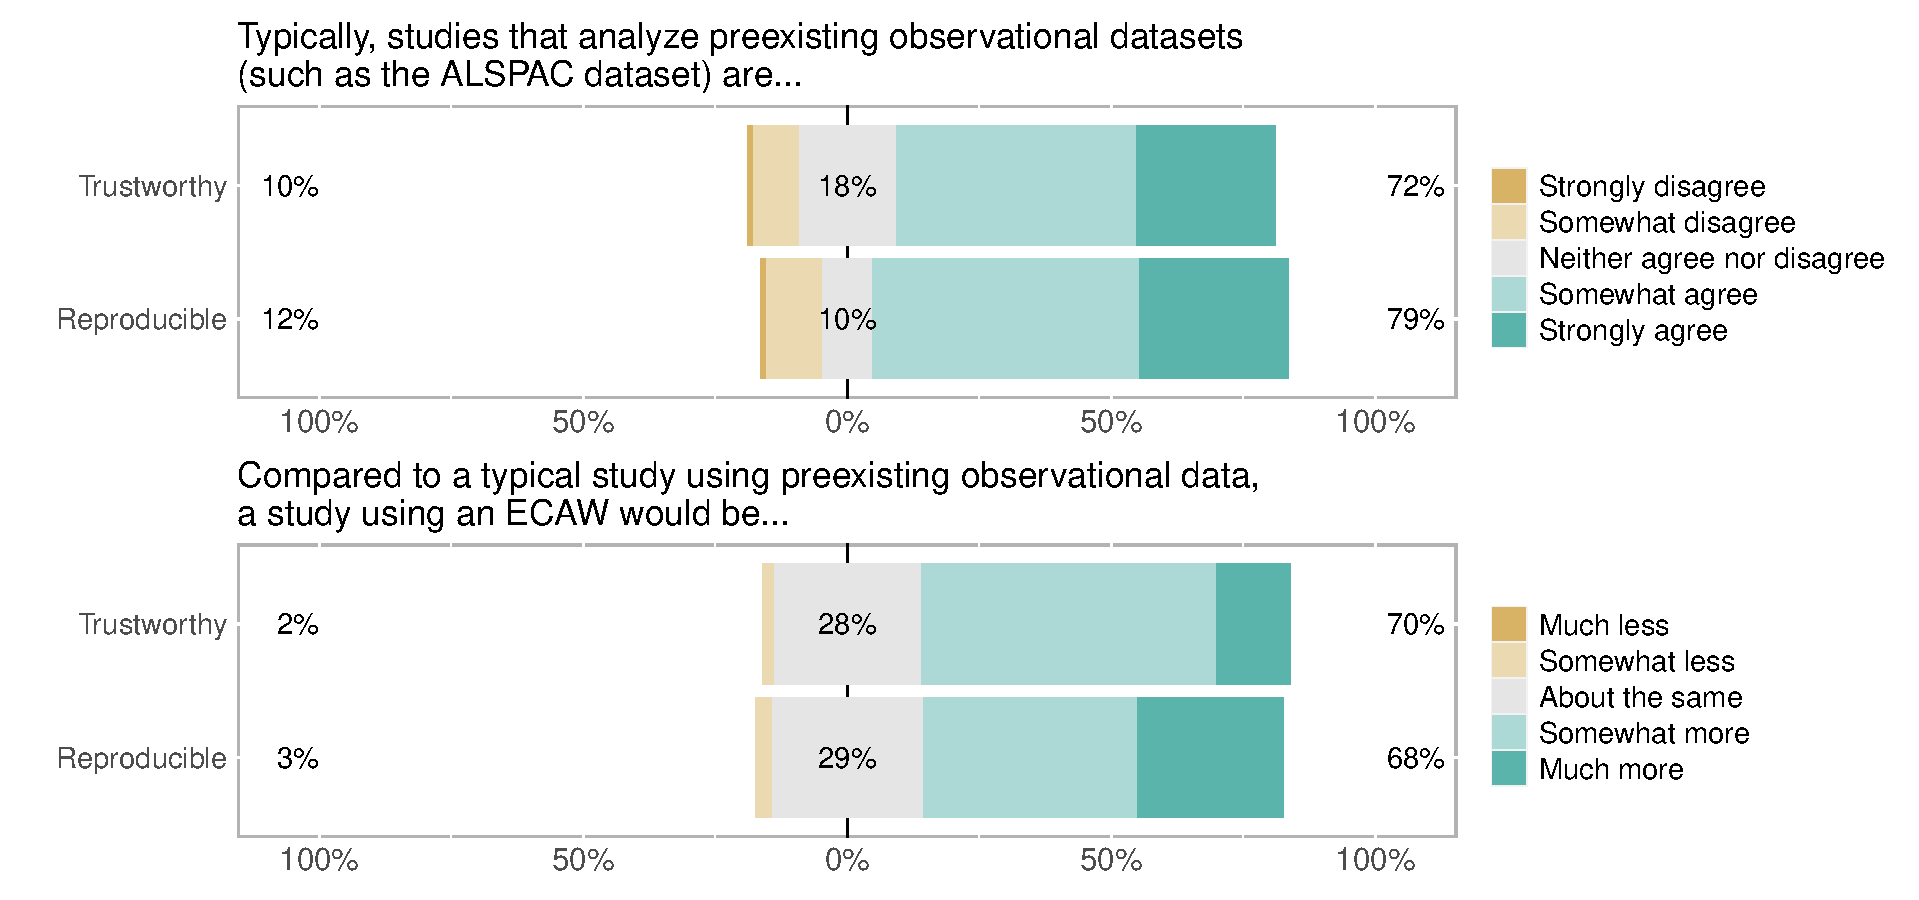
\includegraphics[width=1\linewidth]{figs/typicallyEcawPlot-1} 

}

\caption{\textbf{Figure 1. Responses to the survey questions on trustworthiness and reproducibility of observational research with preexisting data and ECAWs.} The survey defined trustworthy as ``meaning that the results and conclusions of the publications are valid, reliable, rigorous, and accurate. That they merit trust''. The survey defined reproducible ``in the sense that other researchers re-analysing the data with the same research question would produce similar results.'' For each item, the number to the left of the data bar indicates the combined percentage for the responses depicted in any shade of brown/orange. The number in the center of the data bar (gray) indicates the percentage of neutral responses. The number to the right of the data bar indicates the combined percentage for the responses depicted in any shade of green. The bar charts in the top panel had no missing responses or selection of the option \emph{``I don't understand the question''}. The bar charts in the bottom panel excluded responses of \emph{``I don't understand the question''} (n = 3; 2).}\label{fig:typicallyEcawPlot}
\end{figure}

{\smaller[1] \singlespacing



}

Over half of respondents reported that their studies using preexisting observational data are preregistered never or almost never (36\%; 37/103), or sometimes (25\%; 26/103) (Figure 2). About half reported sharing their analysis scripts never or almost never (20\%; 21/103), or sometimes (32\%; 33/103). 77\% (79/103) reported that they never or almost never blind the data analyst. Almost all respondents answered that they use both exploratory (93\%; 96/103) and confirmatory (87\%; 90/103) analyses at least sometimes.

\begin{figure}[H]

{\centering 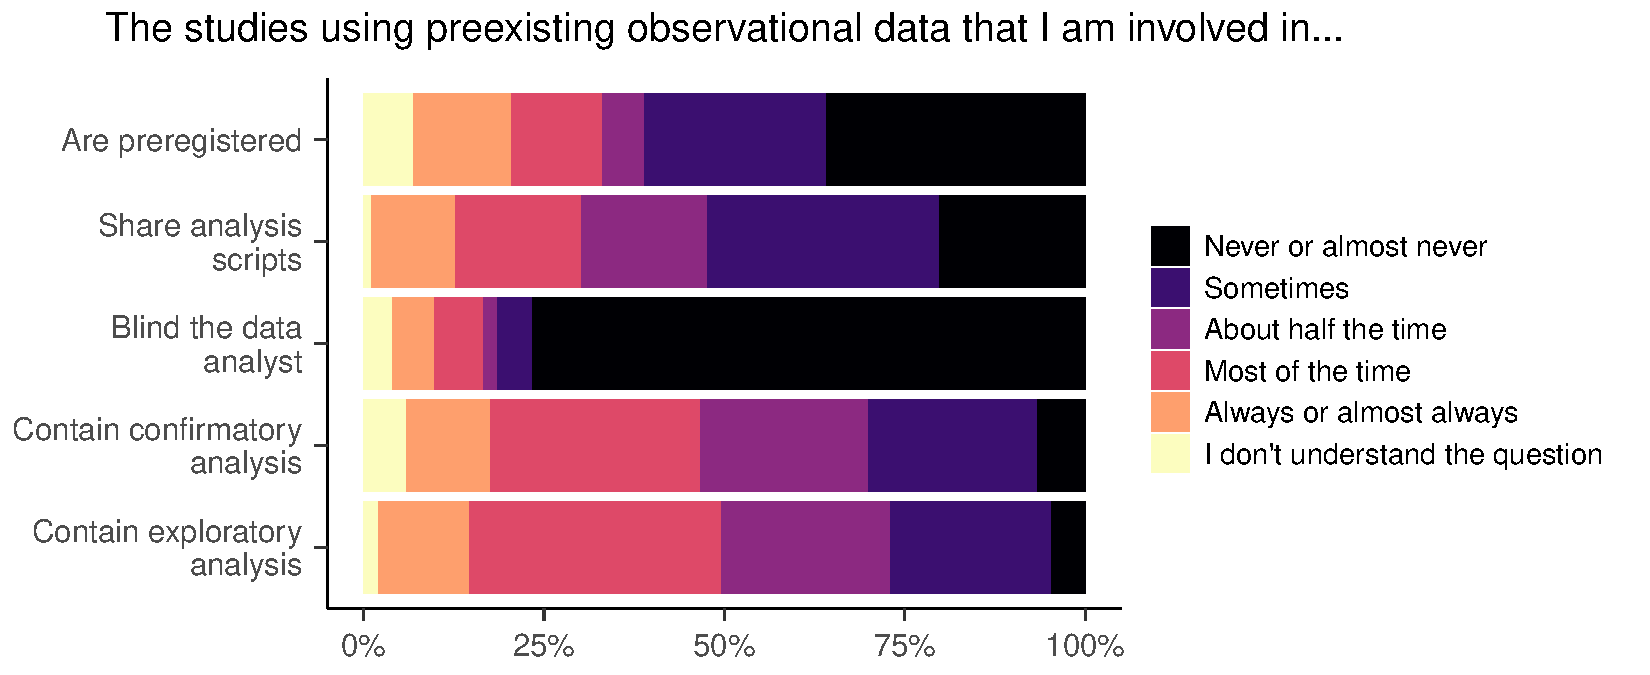
\includegraphics[width=1\linewidth]{figs/methodPlot-1} 

}

\caption{\textbf{Figure 2. Responses to survey questions about the research practices of participants.}}\label{fig:methodPlot}
\end{figure}

{\smaller[1] \singlespacing



}

26\% (26/101) of respondents agreed (versus 45\%; 45/101 who disagreed) that they would be less willing to use ALSPAC data if they were required to use an ECAW (Figure 3). 53\% (50/94) agreed (20\%; 19/94 disagreed) that they would opt-in if ALSPAC ran a study on ECAWs. 55\% (53/96) agreed (10\%; 10/96 disagreed) that ALSPAC should run a study on ECAWs. 46\% (43/94) agreed (22\%; 21/94 disagreed) that they would prefer using an ECAW than using typical preregistration.

\begin{figure}[H]

{\centering 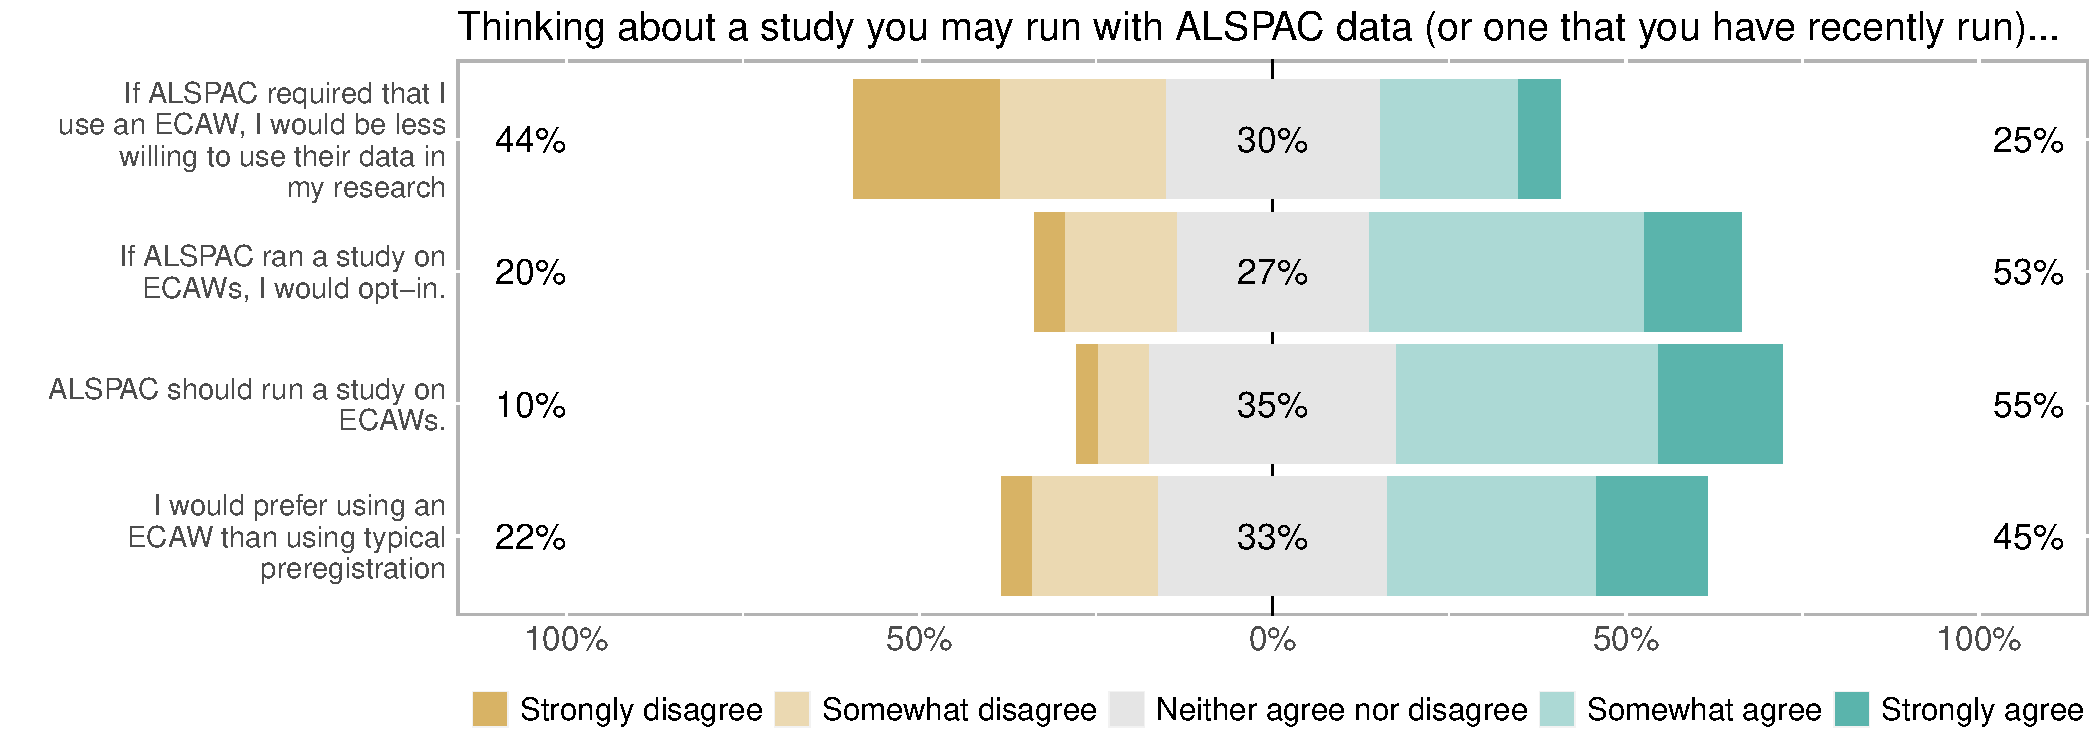
\includegraphics[width=1\linewidth]{figs/alspacPlot-1} 

}

\caption{\textbf{Figure 3. Responses to survey questions about using ECAWs.} These bar charts exclude responses of \emph{``I don't understand the question''} (\emph{n} = 0; 4; 1; 1; respectively from top to bottom), and responses of \emph{``Unsure''} (\emph{n} = 2; 5; 6; 8). Agreement with the first question may be slightly inflated due to the format of the questions in this block. Respondents with a highly positive inclination towards ECAWs would be expected to disagree with the first question, but agree with the next three questions. Four respondents agreed with all four statements, suggesting they may have glazed over the word ``less'' in the first question \protect\footnotemark[3]. Interpreting responses to the second and third question come with a degree of ambiguity as the survey did not specify what was meant by the term ``study'' \protect\footnotemark[4].}\label{fig:alspacPlot}
\end{figure}

{\smaller[1] \singlespacing



}

\protect\footnotetext[3]{Another four respondents agreed with at least the first and second question, which appear contradictory. We did not preregister these considerations. More careful wording of these questions could have circumvented the ambiguity in interpreting these seemingly contradictory responses.}
\protect\footnotetext[4]{We intended for these questions to ask about ALSPAC running a trial on ECAWs. However, due to the ambiguity around the terms “study”, some respondents may have interpreted this as a survey, focus group, feasibility, or pilot type of study.}

\pagebreak

{\smaller[1]
\begin{singlespace}

\textbf{\emph{Table 1. Recurring topics in responses to the open-ended survey questions.}} The survey included 4 open-ended questions with broad prompts regarding running a study on ECAWs, benefits and drawbacks of ECAWs, related research practices, and general comments. These questions received a total of (92) responses from (55) unique respondents. A complete list of responses are viewable in the open data {[}LINK{]}. We synthesized the responses to open-ended questions into the 9 topics on the left side of this table. We divide these into three sections: (i) concerns about the acceptability of ECAWs, (ii) concerns that ECAWs will not have their intended impact, and (iii) alternative interventions that may achieve similar goals as conventional preregistration and ECAWs. On the right side of the table, we provide our reflection on each topic.

\end{singlespace}
}

\begin{figure}

{\centering 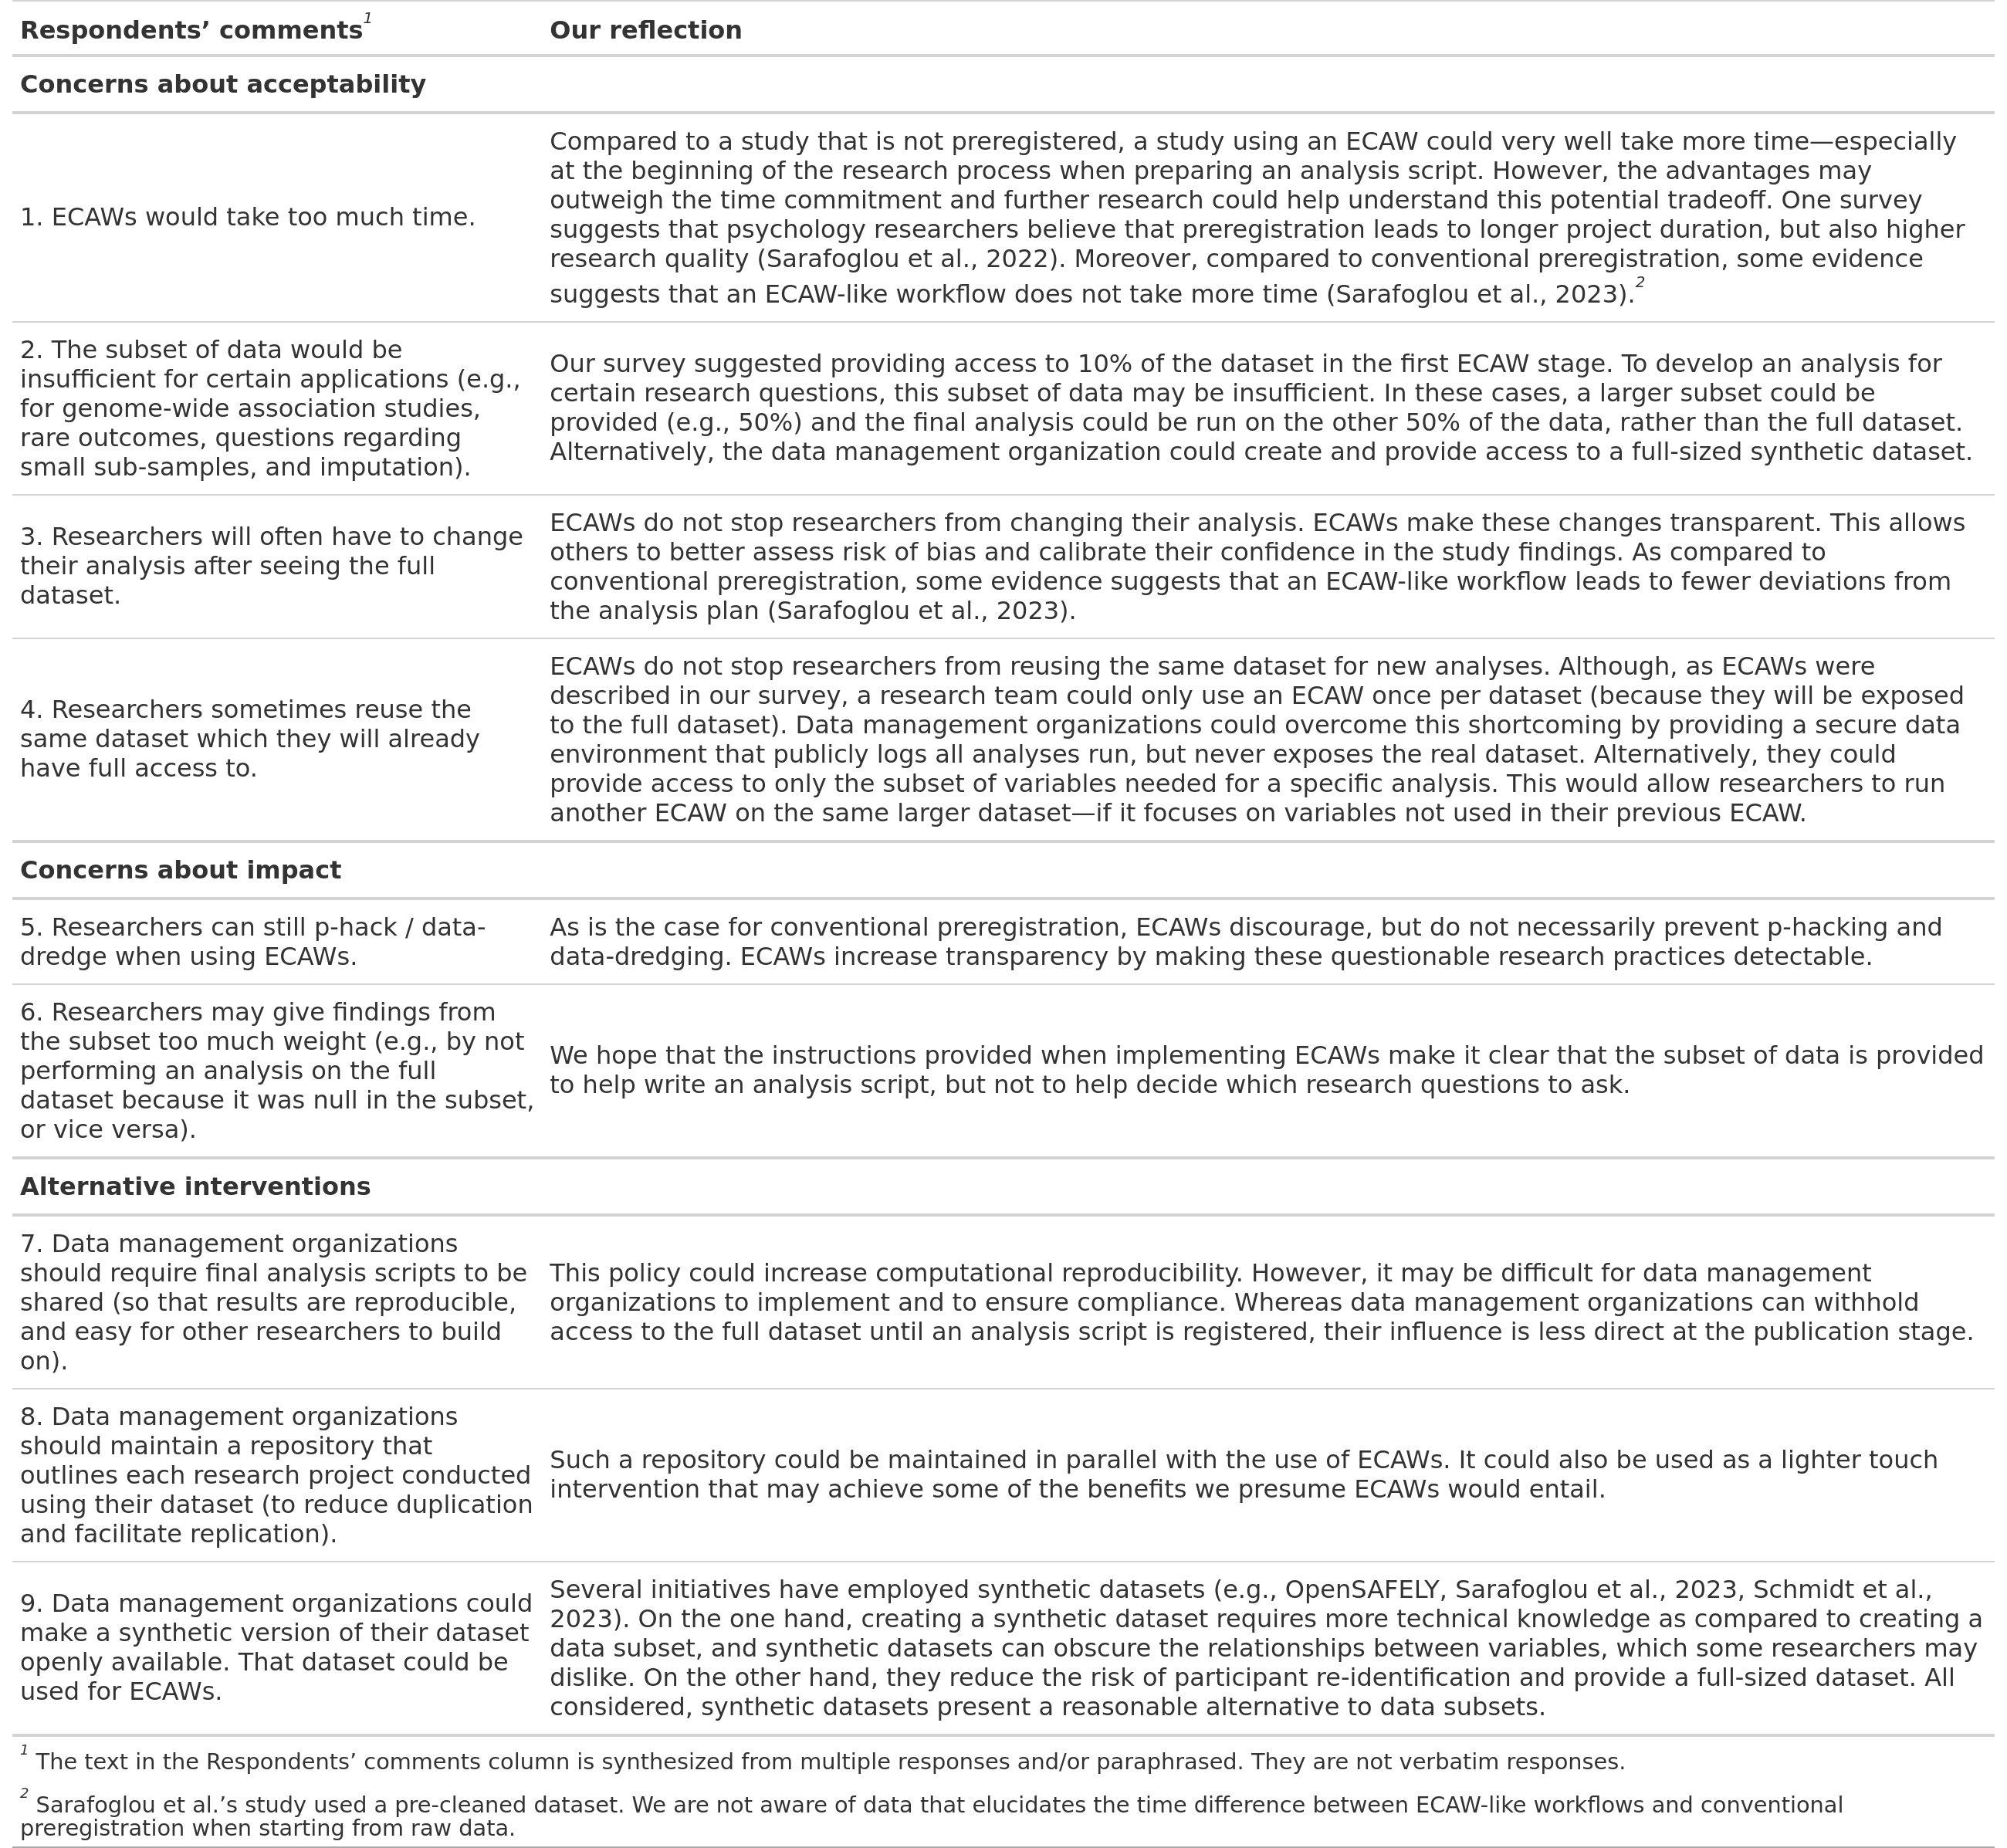
\includegraphics[width=1\linewidth,height=3\textheight]{figs/open-ended-table_figure} 

}

\caption{ }\label{fig:openEndedTable}
\end{figure}

\pagebreak

\hypertarget{exploratory-analyses}{%
\subsection{Exploratory analyses}\label{exploratory-analyses}}

Results can be explored interactively by following the instructions for running the code at {[}INSERT DATA LINK{]}. Based on the sample size of 107 participants and a lack of visually striking differences when exploring subsets of respondents, we do not report further on exploratory analyses.

\hypertarget{discussion}{%
\section{Discussion}\label{discussion}}

The survey results suggest that a trial of ECAWs with ALSPAC could be feasible for at least three reasons. First, ECAWs are possible because most respondents reported performing confirmatory analyses with analysis scripts written using programming languages. Second, ECAWs are relevant because many respondents reported limited use of other methods to improve rigour and reproducibility---including preregistration, sharing analysis scripts, and blinding analysts. Moreover, although participants generally agreed that findings from observational research using pre-existing data are trustworthy and reproducible, they also believed that ECAWs would make research findings more trustworthy and more reproducible. Third, ECAWs appear relatively acceptable. For example, only 10\% of respondents disagreed that ALSPAC should run a study on ECAWs, and 25\% agreed that they would be less likely to use the ALSPAC dataset if they were required to use an ECAW.

The open-ended responses revealed interest in policies and interventions with similar goals to ECAWs. These include requirements for the sharing of final analysis scripts, a database of all ongoing studies that use a particular dataset, and openly available synthetic datasets.

\hypertarget{limitations}{%
\subsection{Limitations}\label{limitations}}

Given the response rate of 10\%, our results represent the opinions of a select set of researchers who may be more interested and involved in reproducible research practices. Indeed, respondents themselves believed that they were more concerned about reproducibility than other researchers in their field (Supplementary Figure C2). ECAWs may be less acceptable among non-responders and non-response may be a mark of lack of interest in the concept. Nonetheless, the absolute number of responders suggests that there is an audience of researchers who might be interested to pursue this approach.

The survey results are best understood as the initial thoughts of participants when introduced to the concept of ECAWs. The median response time was 7.2 minutes (IQR: 4.3 to 13.1) for a survey that included over 20 questions and a 500-word description of ECAWs. Thus, it is unlikely that respondents spent much time reflecting on ECAWs and their implications.

We invited researchers from the ALSPAC mailing list which includes researchers across the fields of health and social sciences, but we did not record the specific disciplines in which the respondents were active. Thus, while ECAWs may be more relevant to some disciplines, the present survey does delve into the idiosyncrasies among disciplines.

Data management organizations could vary widely in their implementation of ECAWs. For example, they could perform checks on the analysis scripts to ensure they run and they could require commented analysis scripts with a clear indication of the primary outcomes. Our survey results do not elucidate the best implementation of ECAWs.

\hypertarget{recommendations}{%
\subsection{Recommendations}\label{recommendations}}

Some data management organizations looking to implement ECAWs will need to consider a balance between updating their data access workflow and maintaining their user numbers, engagement, and funding. This consideration will depend heavily on the structure of the data management organization. An organization managing data that is routinely collected somewhat regardless of its potential for use in research (e.g., electronic health records) may have leeway to test new workflows even if they impact user numbers. Other organizations---such as ALSPAC---coordinate ongoing data collection efforts that compound the value of their dataset and their continued operation remains contingent on funding cycles and data access fees. Even if ECAWs led to an increase in user numbers in the long-term, a temporary decrease could preclude the cost recovery systems on which their staff rely. In a more extreme case, the likelihood of another successful funding cycle could be impacted and compromise the project's continuation. Funders and institutions interested in supporting these types of initiatives could alleviate concerns by providing targeted funding for testing these interventions and offering contingency funds to maintain cost recovery systems.

With these considerations in mind, an organization like ALSPAC may benefit from first leveraging the substantial number of respondents who would opt-in to a study on ECAWs. Trialing ECAWs with this user group would allow organizations to collect data that may support more widespread implementation, including project completion time, study quality, and researcher satisfaction when using ECAWs. They could refine the ECAW pipeline with minimal concern about user numbers. In the situation that a data management organization is already considering implementing policies on preregistration, they may benefit from considering alternate workflows such as ECAWs, which many respondents deemed preferable to conventional preregistration. The open-ended responses to our survey also suggest some confusion around the purpose of ECAWs and the process of using them. A clear-cut module provided by data management organizations that explains the ECAW concept alongside step-by-step instructions could help address researchers' concerns preemptively and help them adopt this workflow.

The stakes are lower in cases where a static final dataset already exists and concerns about funding are absent. For example, researchers with an interest in rigorous analyses and who control access to a dataset have already employed ECAW-like workflows (e.g., Forscher et al. (2020); Schmidt et al. (2023)). Concerns about a reduction in user numbers and engagement may also be less relevant for datasets containing unique data. For example, a researcher trying to answer a question about health and development with ALSPAC data, may also be able to answer that question with another cohort dataset. However, a researcher trying to answer a question about the population of a specific country may need access to that country's census data, regardless of the workflow required by that data management organization. A final consideration is that user numbers and engagement may increase if researchers feel that ECAWs increase the trustworthiness of their findings and others come to associate research from datasets using ECAWs as more open and rigorous.

\hypertarget{conclusion}{%
\subsection{Conclusion}\label{conclusion}}

In this manuscript, we outlined a research workflow---ECAW---which necessitates certain open science practices and can be implemented by data management organizations. Responses to our survey provide information for organizations interested in developing and testing ECAWs and interventions with related goals.

\begin{center}\rule{0.5\linewidth}{0.5pt}\end{center}

\hypertarget{ethical-approval}{%
\subsection{Ethical approval}\label{ethical-approval}}

Ethical approval for the study was obtained from the ALSPAC Ethics and Law Committee and the Faculty of Life Sciences Research Ethics Committee at the University of Bristol (approval code: 12260).

\hypertarget{acknowledgements}{%
\subsection{Acknowledgements}\label{acknowledgements}}

We thank Nicholas Timpson and Kate Northstone for invaluable input throughout this research project. We thank the ALSPAC Executive for their collaboration and willingness to run this study. We thank all the participants for their responses.

\hypertarget{funding}{%
\subsection{Funding}\label{funding}}

Robert Thibault is supported by a general support grant awarded to METRICS from Arnold Ventures and a postdoctoral fellowship from the Canadian Institutes of Health Research. Alexandra Sarafoglou was supported by an Amsterdam Brain and Cognition project grant (grant ref: ABC PG 22 - January 2022) ``From rigid theory to cognitive models: a framework to study individual differences in meaning representations'\,'. The UK Medical Research Council and Wellcome (Grant ref: 217065/Z/19/Z) and the University of Bristol provide core support for ALSPAC. This publication is the work of the authors and Robert Thibault will serve as guarantor for the contents of this paper. The funders have no role in the preparation of this manuscript or the decision to publish.

\hypertarget{contributions}{%
\subsection{Contributions}\label{contributions}}

\textbf{Conceptualization:} Robert T. Thibault and Marcus R. Munafò.\hfill\break
\textbf{Data curation:} Marton Kovacs.\hfill\break
\textbf{Formal analysis:} Robert T. Thibault and Marton Kovacs.\hfill\break
\textbf{Funding acquisition:} Robert T. Thibault and John P. A. Ioannidis.\hfill\break
\textbf{Investigation:} Robert T. Thibault.\hfill\break
\textbf{Methodology:} Robert T. Thibault, Tom E. Hardwicke, Alexandra Sarafoglou, John P. A. Ioannidis, and Marcus R. Munafò.\hfill\break
\textbf{Project administration:} Robert T. Thibault.\hfill\break
\textbf{Resources:} Robert T. Thibault.\hfill\break
\textbf{Software:} Marton Kovacs.\hfill\break
\textbf{Supervision:} Robert T. Thibault and Marcus R. Munafò.\hfill\break
\textbf{Validation:} Robert T. Thibault and Marton Kovacs.\hfill\break
\textbf{Visualization:} Robert T. Thibault and Marton Kovacs.\hfill\break
\textbf{Writing - original draft:} Robert T. Thibault.\hfill\break
\textbf{Writing - review \& editing:} Robert T. Thibault, Marton Kovacs, Tom E. Hardwicke, Alexandra Sarafoglou, John P. A. Ioannidis, and Marcus R. Munafò.

\hypertarget{competing-interests}{%
\subsection{Competing interests}\label{competing-interests}}

All authors declare no conflict of interest.

\newpage

\hypertarget{references}{%
\section{References}\label{references}}

\hypertarget{refs}{}
\begin{CSLReferences}{1}{0}
\leavevmode\vadjust pre{\hypertarget{ref-bakker_ensuring_2020}{}}%
Bakker, M., Veldkamp, C. L., Assen, M. A. van, Crompvoets, E. A., Ong, H. H., Nosek, B. A., \ldots{} Wicherts, J. M. (2020). Ensuring the quality and specificity of preregistrations. \emph{PLoS Biology}, \emph{18}(12), e3000937.

\leavevmode\vadjust pre{\hypertarget{ref-camerer_evaluating_2016}{}}%
Camerer, C. F., Dreber, A., Forsell, E., Ho, T.-H., Huber, J., Johannesson, M., \ldots{} Chan, T. (2016). Evaluating replicability of laboratory experiments in economics. \emph{Science}, \emph{351}(6280), 1433--1436.

\leavevmode\vadjust pre{\hypertarget{ref-collaboration_estimating_2015}{}}%
Collaboration, O. S. (2015). Estimating the reproducibility of psychological science. \emph{Science}, \emph{349}(6251), aac4716.

\leavevmode\vadjust pre{\hypertarget{ref-errington_investigating_2021}{}}%
Errington, T. M., Mathur, M., Soderberg, C. K., Denis, A., Perfito, N., Iorns, E., \& Nosek, B. A. (2021). Investigating the replicability of preclinical cancer biology. \emph{Elife}, \emph{10}, e71601.

\leavevmode\vadjust pre{\hypertarget{ref-Forscher2020}{}}%
Forscher, P. S., Noyce, A., DeBruine, L. M., Jones, B., Flake, J. K., Coles, N. A., \& Chartier, C. R. (2020). \emph{Incentivizing discovery through the {PSA001} secondary analysis challenge}. \url{https://psysciacc.org/2020/09/14/incentivizing-discovery-through-the-psa001-secondary-analysis-challenge/}.

\leavevmode\vadjust pre{\hypertarget{ref-ioannidis_why_2005}{}}%
Ioannidis, J. P. (2005). Why most published research findings are false. \emph{PLoS Medicine}, \emph{2}(8), e124.

\leavevmode\vadjust pre{\hypertarget{ref-ioannidis_why_2008}{}}%
Ioannidis, J. P. (2008). Why most discovered true associations are inflated. \emph{Epidemiology}, 640--648.

\leavevmode\vadjust pre{\hypertarget{ref-klein_blind_2005}{}}%
Klein, J. R., \& Roodman, A. (2005). Blind analysis in nuclear and particle physics. \emph{Annu. Rev. Nucl. Part. Sci.}, \emph{55}, 141--163.

\leavevmode\vadjust pre{\hypertarget{ref-maccoun_blind_2015}{}}%
MacCoun, R., \& Perlmutter, S. (2015). Blind analysis: {Hide} results to seek the truth. \emph{Nature}, \emph{526}(7572), 187--189.

\leavevmode\vadjust pre{\hypertarget{ref-prasad_ending_2019}{}}%
Prasad, V. K., \& Cifu, A. S. (2019). \emph{Ending medical reversal: Improving outcomes, saving lives}. Johns Hopkins University Press.

\leavevmode\vadjust pre{\hypertarget{ref-sarafoglou_comparing_2023}{}}%
Sarafoglou, A., Hoogeveen, S., \& Wagenmakers, E.-J. (2023). Comparing analysis blinding with preregistration in the many-analysts religion project. \emph{Advances in Methods and Practices in Psychological Science}, \emph{6}(1), 25152459221128319.

\leavevmode\vadjust pre{\hypertarget{ref-Schmidt2023}{}}%
Schmidt, K., Jones, A., Szabelska, A., Ebersole, C. R., Hawkins, C. B., Graham, J., \& Nosek, B. A. (2023). \emph{The ideology 2.0 study and dataset}. \url{https://osf.io/2483h/wiki/home/}; OSF.

\end{CSLReferences}

\newpage

\hypertarget{supplementary-material-a.-deviations-from-the-preregistration.}{%
\section{Supplementary Material A. Deviations from the preregistration.}\label{supplementary-material-a.-deviations-from-the-preregistration.}}

\begin{enumerate}

  \item We rephrased our second objective to be more accurate. The preregistration reads “2.    To use these insights to inform future research on how data management organizations can encourage rigorous and reproducible research practices (survey Blocks 3-6). This objective includes assessing and refining potential interventions—such as ECAWs—and assessing their acceptability. ”. The manuscript reads “(2) To use these insights to inform future research—including a potential trial of ECAWs with the Avon Longitudinal Study of Parents and Children (ALSPAC)—on how data management organizations can encourage rigorous and reproducible research practices.”
  \item Marton Kovacs was added as a contributor during data collection. This led to a few of the projected contributor roles outlined in the preregistration to be different from the final contributor roles outlined in the manuscript.
  \item The preregistration stated that: “We will tabulate descriptive summary statistics for all the survey questions.” Instead of tabulating the results, the manuscript presents this data in figures. We feel that the figures are easier to digest as compared to tabulated data.
  \item The preregistration stated that: “we   will   present   results   that   include   responses   from participants who did not complete the entire survey, alongside the associated response rate for each question.”. The results from all participants are presented in Supplementary Material D. However, instead of reporting the associated response rate for each question, we simply state that “The survey was completed 107 times and partially completed 27 times, leading to a response rate of 10% for complete surveys and 12% for incomplete surveys.”
  \item The preregistration and survey use the term “typical preregistration”. We changed this to “conventional preregistration” in the manuscript because we believe it is the more appropriate term.
  \item We performed a brief visual inspection of the data presented in spreadsheet format. Three participants clicked through to the end of the survey—so they were coded as completing the survey—however, they only responded to a few of the first questions. One other participant appears to have provided non-sincere responses in that all their responses were neutral or skipped and they completed the survey in 146 seconds. We retained these four participants as partially completed responses (results in Supplementary Material D), but removed them from the main dataset. These decisions were not preregistered.
  \item We did not preregister which results we would present in the abstract. We decided to report the results with the highest and lowest percentage about the acceptability of ECAWs: “For example, only 10\% of respondents disagreed that ALSPAC should run a study on ECAWs, but as many as 25\% of respondents agreed they would be less willing to use ALSPAC data if they were required to use an ECAW.”

\end{enumerate}

\pagebreak

\hypertarget{supplementary-material-b.-invitation-email}{%
\section{Supplementary Material B. Invitation email}\label{supplementary-material-b.-invitation-email}}

\hypertarget{original-email}{%
\subsection{Original email}\label{original-email}}

Dear ALSPAC Data User,

We are working with Dr Robert Thibault, a postdoctoral scholar at Stanford University and the University of Bristol, to support his work on scientific rigour and reproducibility in observational studies.

To assist him in his research we would be very grateful if you would consider completing a short survey. The purpose of this is to understand researcher's practices and thoughts regarding the rigour and reproducibility of observational research that uses pre-existing datasets (such as the ALSPAC resource). Results from this survey may be used in the future to inform initiatives for ALSPAC to better serve our users and to maximise the quality of the research using ALSPAC.

The survey has 21 questions across six sections. It will be open until November 1 at this link: \url{https://bristolexppsych.eu.qualtrics.com/jfe/form/SV_3mVgk4lzXx4kp02}. It will take approximately 10-20 minutes to complete. The data you provide is completely anonymous and further information is available on the consent form at the start of the survey.

If you have any questions or comments, please send them directly to Robert (\href{mailto:robert.thibault@bristol.ac.uk}{\nolinkurl{robert.thibault@bristol.ac.uk}}).

Kind regards,

The ALSPAC Executive

\begin{center}\rule{0.5\linewidth}{0.5pt}\end{center}

\hypertarget{first-follow-up-email-sent-after-1-week}{%
\subsection{First follow-up email (sent after 1 week)}\label{first-follow-up-email-sent-after-1-week}}

Dear ALSPAC data user,

Thank you very much to those of you who have already completed the survey below.
There is still time to complete the survey (see details in the original email below), which closes on November 1st.

Please send any comments or queries directly to Robert (\href{mailto:robert.thibault@bristol.ac.uk}{\nolinkurl{robert.thibault@bristol.ac.uk}}).

Many thanks,

The ALSPAC Executive

\begin{center}\rule{0.5\linewidth}{0.5pt}\end{center}

\hypertarget{second-follow-up-email-sent-after-2-weeks}{%
\subsection{Second follow-up email (sent after 2 weeks)}\label{second-follow-up-email-sent-after-2-weeks}}

Dear ALSPAC data user,

Thank you very much to those of you who have already completed the survey below.
This will be our final email inviting you to complete the survey (see details in the original email below), which closes of November 1st.

The median time to complete the survey has been 8 minutes.

Please send any comments or queries directly to Robert (\href{mailto:robert.thibault@bristol.ac.uk}{\nolinkurl{robert.thibault@bristol.ac.uk}}).

Many thanks,
The ALSPAC Executive

\pagebreak

\hypertarget{supplementary-material-c.-participant-characteristics}{%
\section{Supplementary Material C. Participant Characteristics}\label{supplementary-material-c.-participant-characteristics}}

\begin{figure}

{\centering 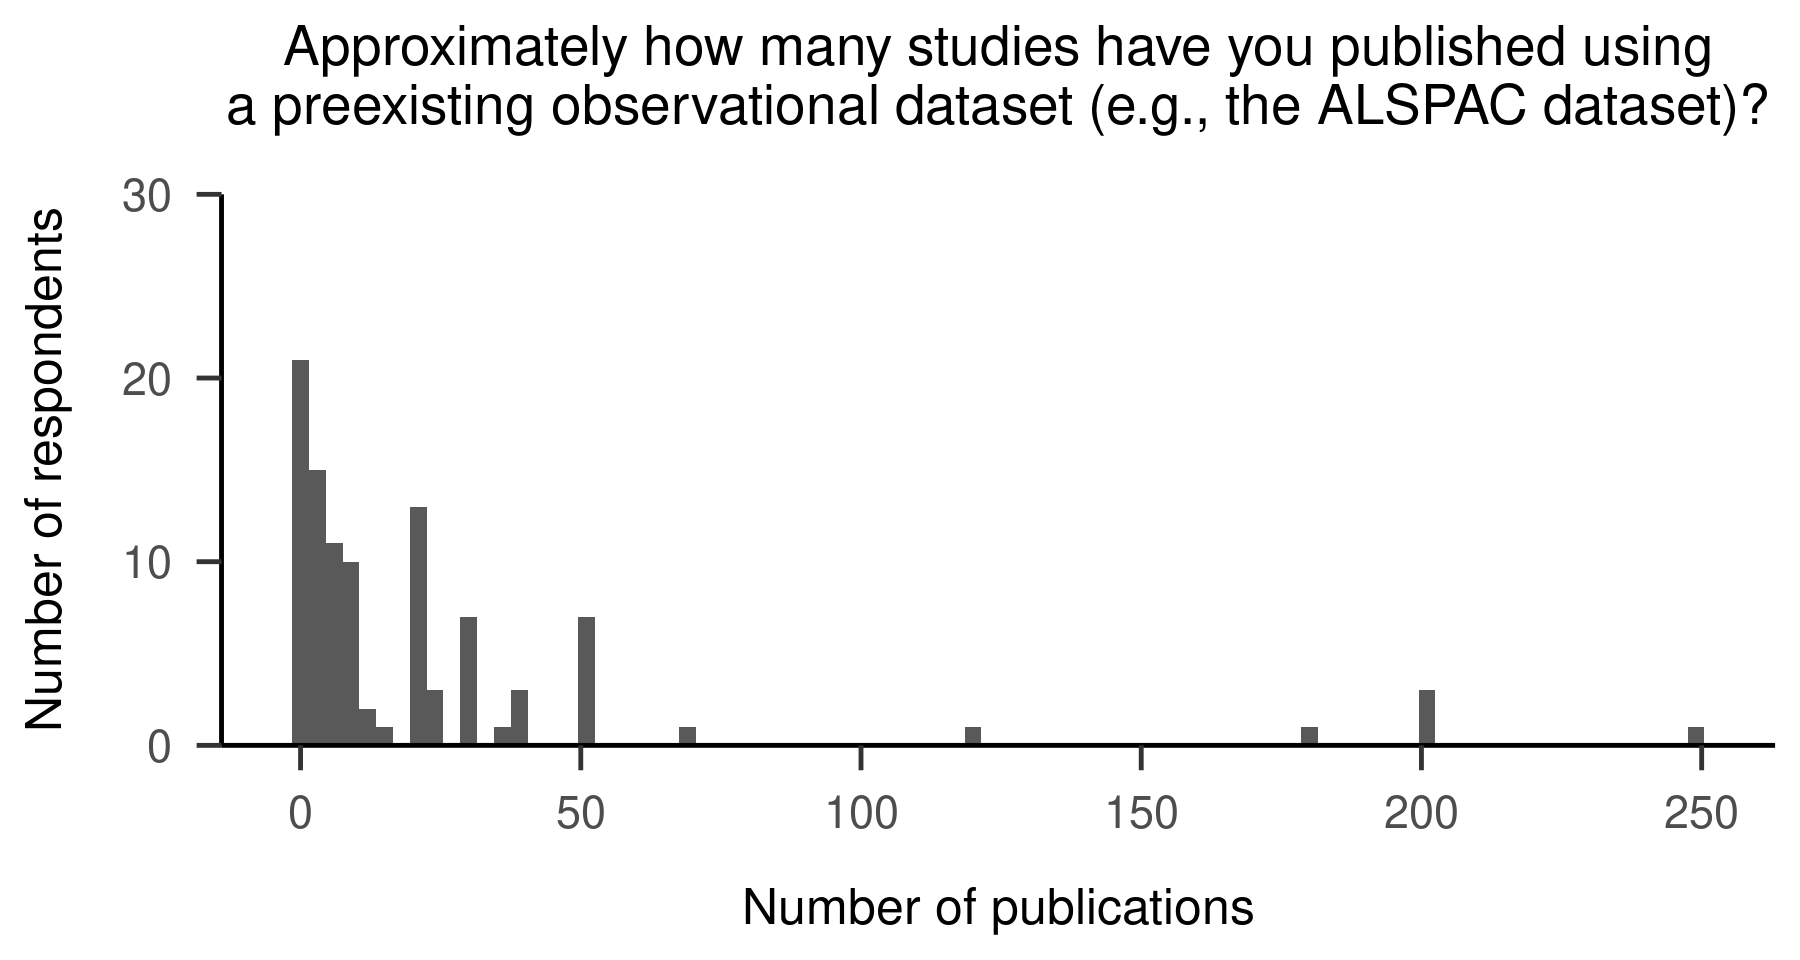
\includegraphics[width=1\linewidth]{figs/numStudiesPlot-1} 

}

\caption{\textbf{Figure C1.}}\label{fig:numStudiesPlot}
\end{figure}

{\smaller[1]
\begin{singlespace}



\end{singlespace}
}

\begin{table}[H]

\caption{\label{tab:languageTable}\textbf{Table C1. ``What programming language or software do you use for your analyses of preexisting observational data? (you may select multiple answers)''}}
\resizebox{\linewidth}{!}{
\begin{tabular}[t]{lrr}
\toprule
\textbf{Programming language} & \textbf{N} & \textbf{Percentage of respondents}\\
\midrule
R & 65 & 63\\
\cmidrule{1-3}
Stata & 48 & 47\\
\cmidrule{1-3}
SPSS & 17 & 17\\
\cmidrule{1-3}
SAS & 15 & 15\\
\cmidrule{1-3}
Python & 6 & 6\\
\cmidrule{1-3}
Mplus & 3 & 3\\
\cmidrule{1-3}
Bash & 2 & 2\\
\cmidrule{1-3}
MATLAB & 1 & 1\\
\cmidrule{1-3}
Nextflow & 1 & 1\\
\cmidrule{1-3}
plink2 & 1 & 1\\
\bottomrule
\end{tabular}}
\end{table}

{\smaller[1]
\begin{singlespace}



\end{singlespace}
}

\begin{figure}

{\centering 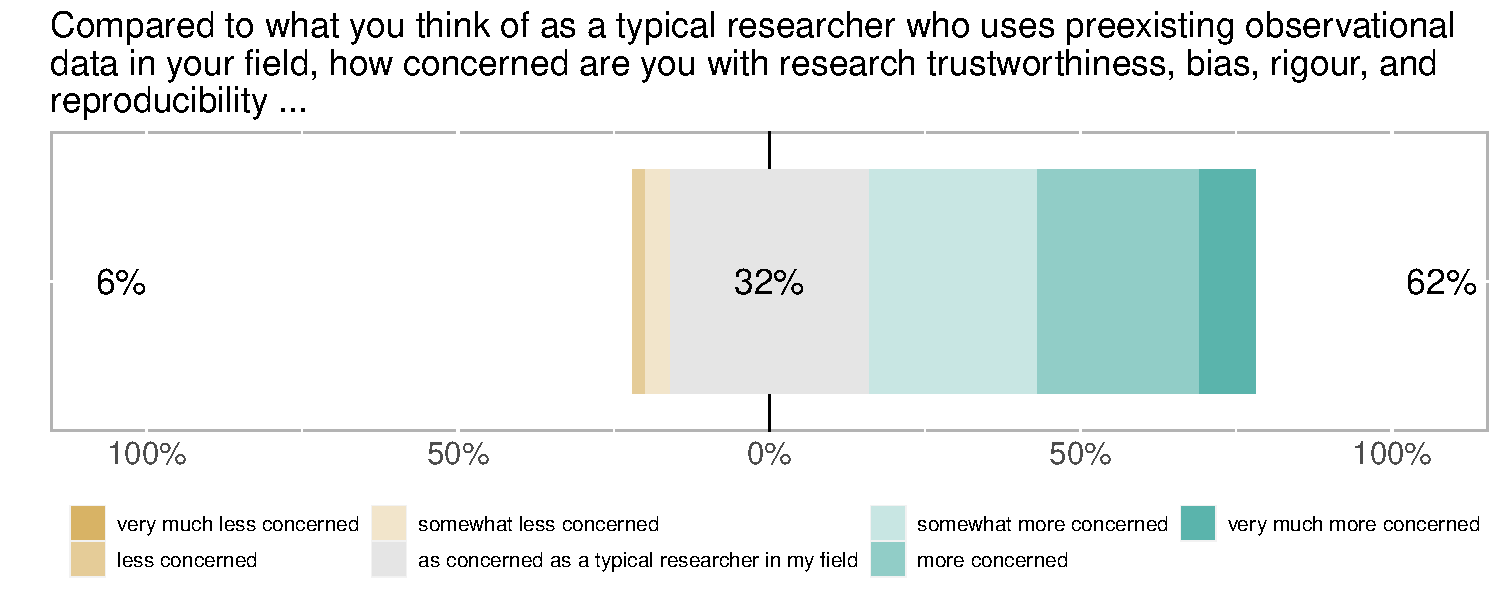
\includegraphics[width=1\linewidth]{figs/concernedPlot-1} 

}

\caption{\textbf{Figure C2. Responses to survey question about number of relevant publications}}\label{fig:concernedPlot}
\end{figure}

{\smaller[1]
\begin{singlespace}



\end{singlespace}
}

\pagebreak

\hypertarget{supplementary-material-d.-figures-and-tables-including-participants-who-partially-complete-the-survey}{%
\section{Supplementary Material D. Figures and Tables including participants who partially complete the survey}\label{supplementary-material-d.-figures-and-tables-including-participants-who-partially-complete-the-survey}}

\hypertarget{participants-2}{%
\subsection{Participants}\label{participants-2}}

Respondents had published a median of 10 (IQR 2 to 25) studies using preexisting observational data. They reported using the following programming languages or software packages: R (n = 65), Stata (n = 48), SPSS (n = 17), SAS (n = 15), Python (n = 6), Mplus (n = 3), Bash (n = 2), MATLAB (n = 1), Nextflow (n = 1), and plink2 (n = 1) \footnote[1]{Participants could select multiple responses to this survey question.}. 61\% (62/101) of participants reported being more concerned with research trustworthiness, bias, rigour, and reproducibility compared to what they think of as a typical research who uses preexisting observational data; 6\% (6/101) reported being less concerned.

\hypertarget{survey-results-1}{%
\subsection{Survey results}\label{survey-results-1}}

Most respondents agreed that studies that analyze preexisting observational datasets are trustworthy (71\%; 87/123) and reproducible (77\%; 93/121) (Figure D2, top panel). At the same time, many agreed that a study using an ECAW would be \emph{more} trustworthy (70\%; 70/107) and \emph{more} reproducible (69\%; 74/108) compared to a typical study using preexisting observational data (Figure 1, bottom panel).

\begin{figure}[H]

{\centering 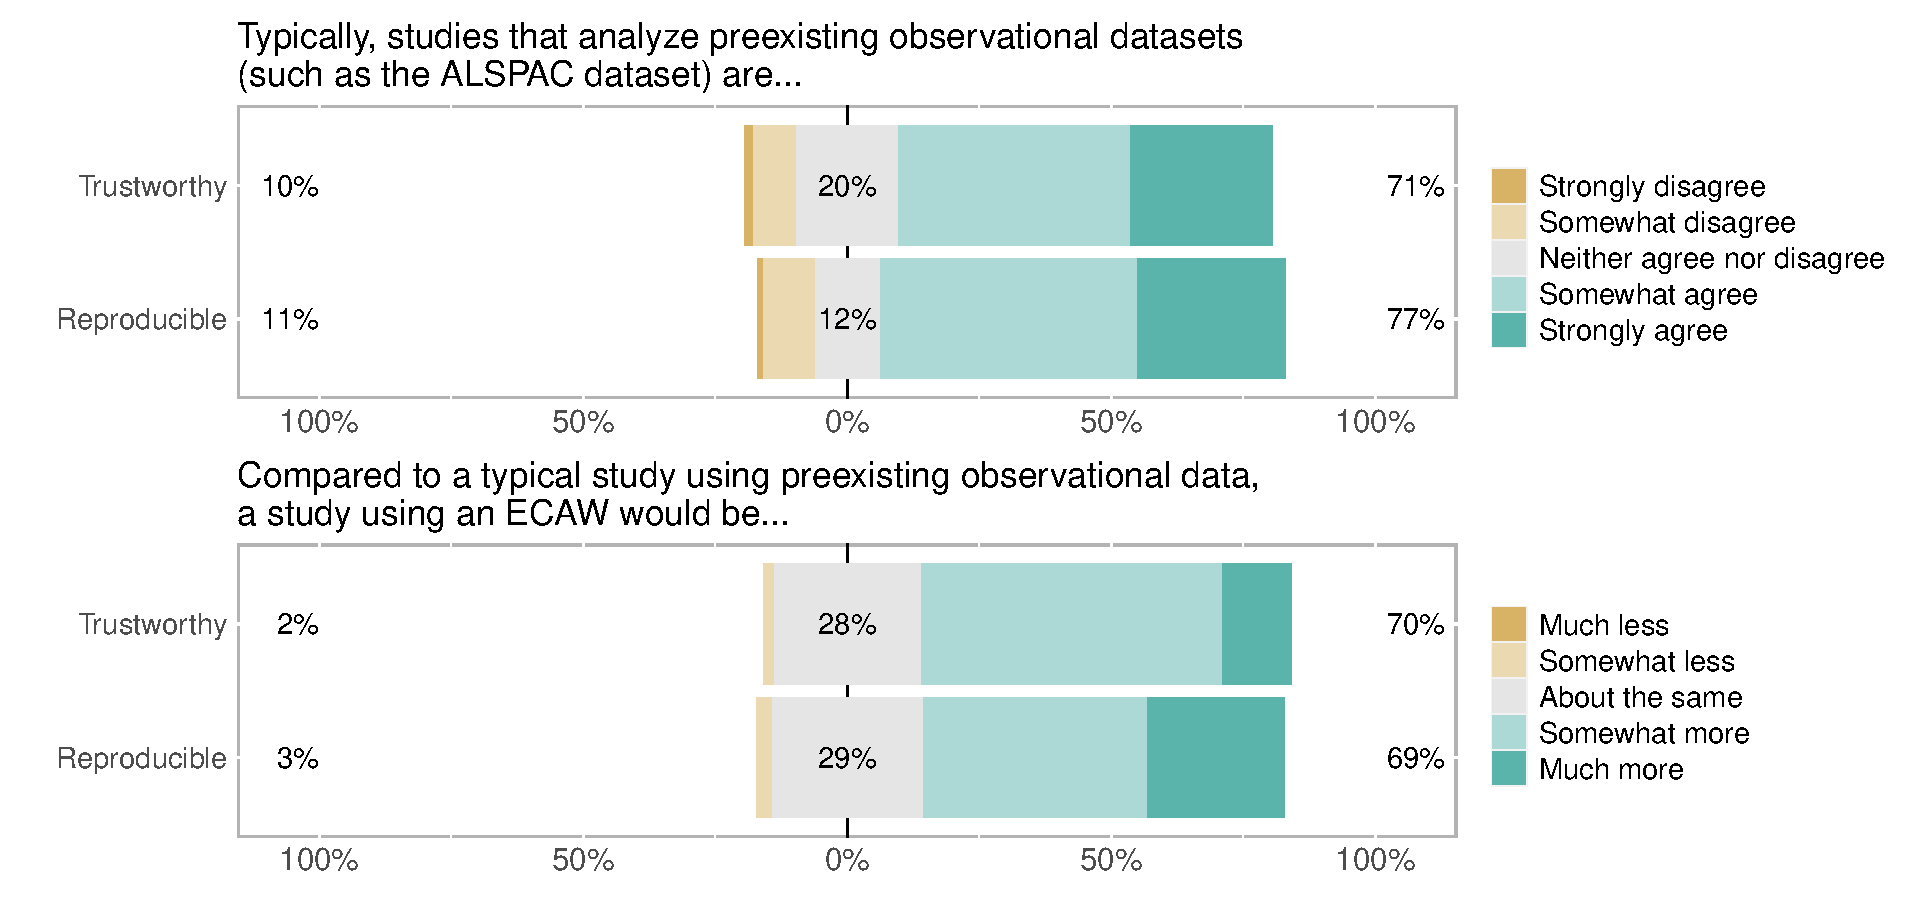
\includegraphics[width=1\linewidth]{figs/typicallyEcawPlotAll-1} 

}

\caption{\textbf{Figure 1D. Responses to the survey questions on trustworthiness and reproducibility of observational research with preexisting data and ECAWs.} The survey defined trustworthy as ``meaning that the results and conclusions of the publications are valid, reliable, rigorous, and accurate. That they merit trust''. The survey defined reproducible ``in the sense that other researchers re-analysing the data with the same research question would produce similar results.'' For each item, the number to the left of the data bar indicates the combined percentage for the responses depicted in any shade of brown/orange. The number in the center of the data bar (gray) indicates the percentage of neutral responses. The number to the right of the data bar indicates the combined percentage for the responses depicted in any shade of green. The bar charts in the top panel had no missing responses or selection of the option \emph{``I don't understand the question''}. The bar charts in the bottom panel excluded missing responses (n = 12; 12) and responses of \emph{``I don't understand the question''} (n = 4; 3).}\label{fig:typicallyEcawPlotAll}
\end{figure}

{\smaller[1]
\begin{singlespace}



\end{singlespace}
}

Over half of respondents reported that their studies using preexisting observational data are preregistered never or almost never (33\%; 41/123), or sometimes (21\%; 26/103) (Figure 2D). About half reported sharing their analysis scripts never or almost never (19\%; 23/123), or sometimes (29\%; 36/123). 69\% (85/123) reported that they never or almost never blind the data analyst. Almost all respondents answered that they use both exploratory (87\%; 107/123) and confirmatory (82\%; 101/123) analyses at least sometimes.

\begin{figure}[H]

{\centering 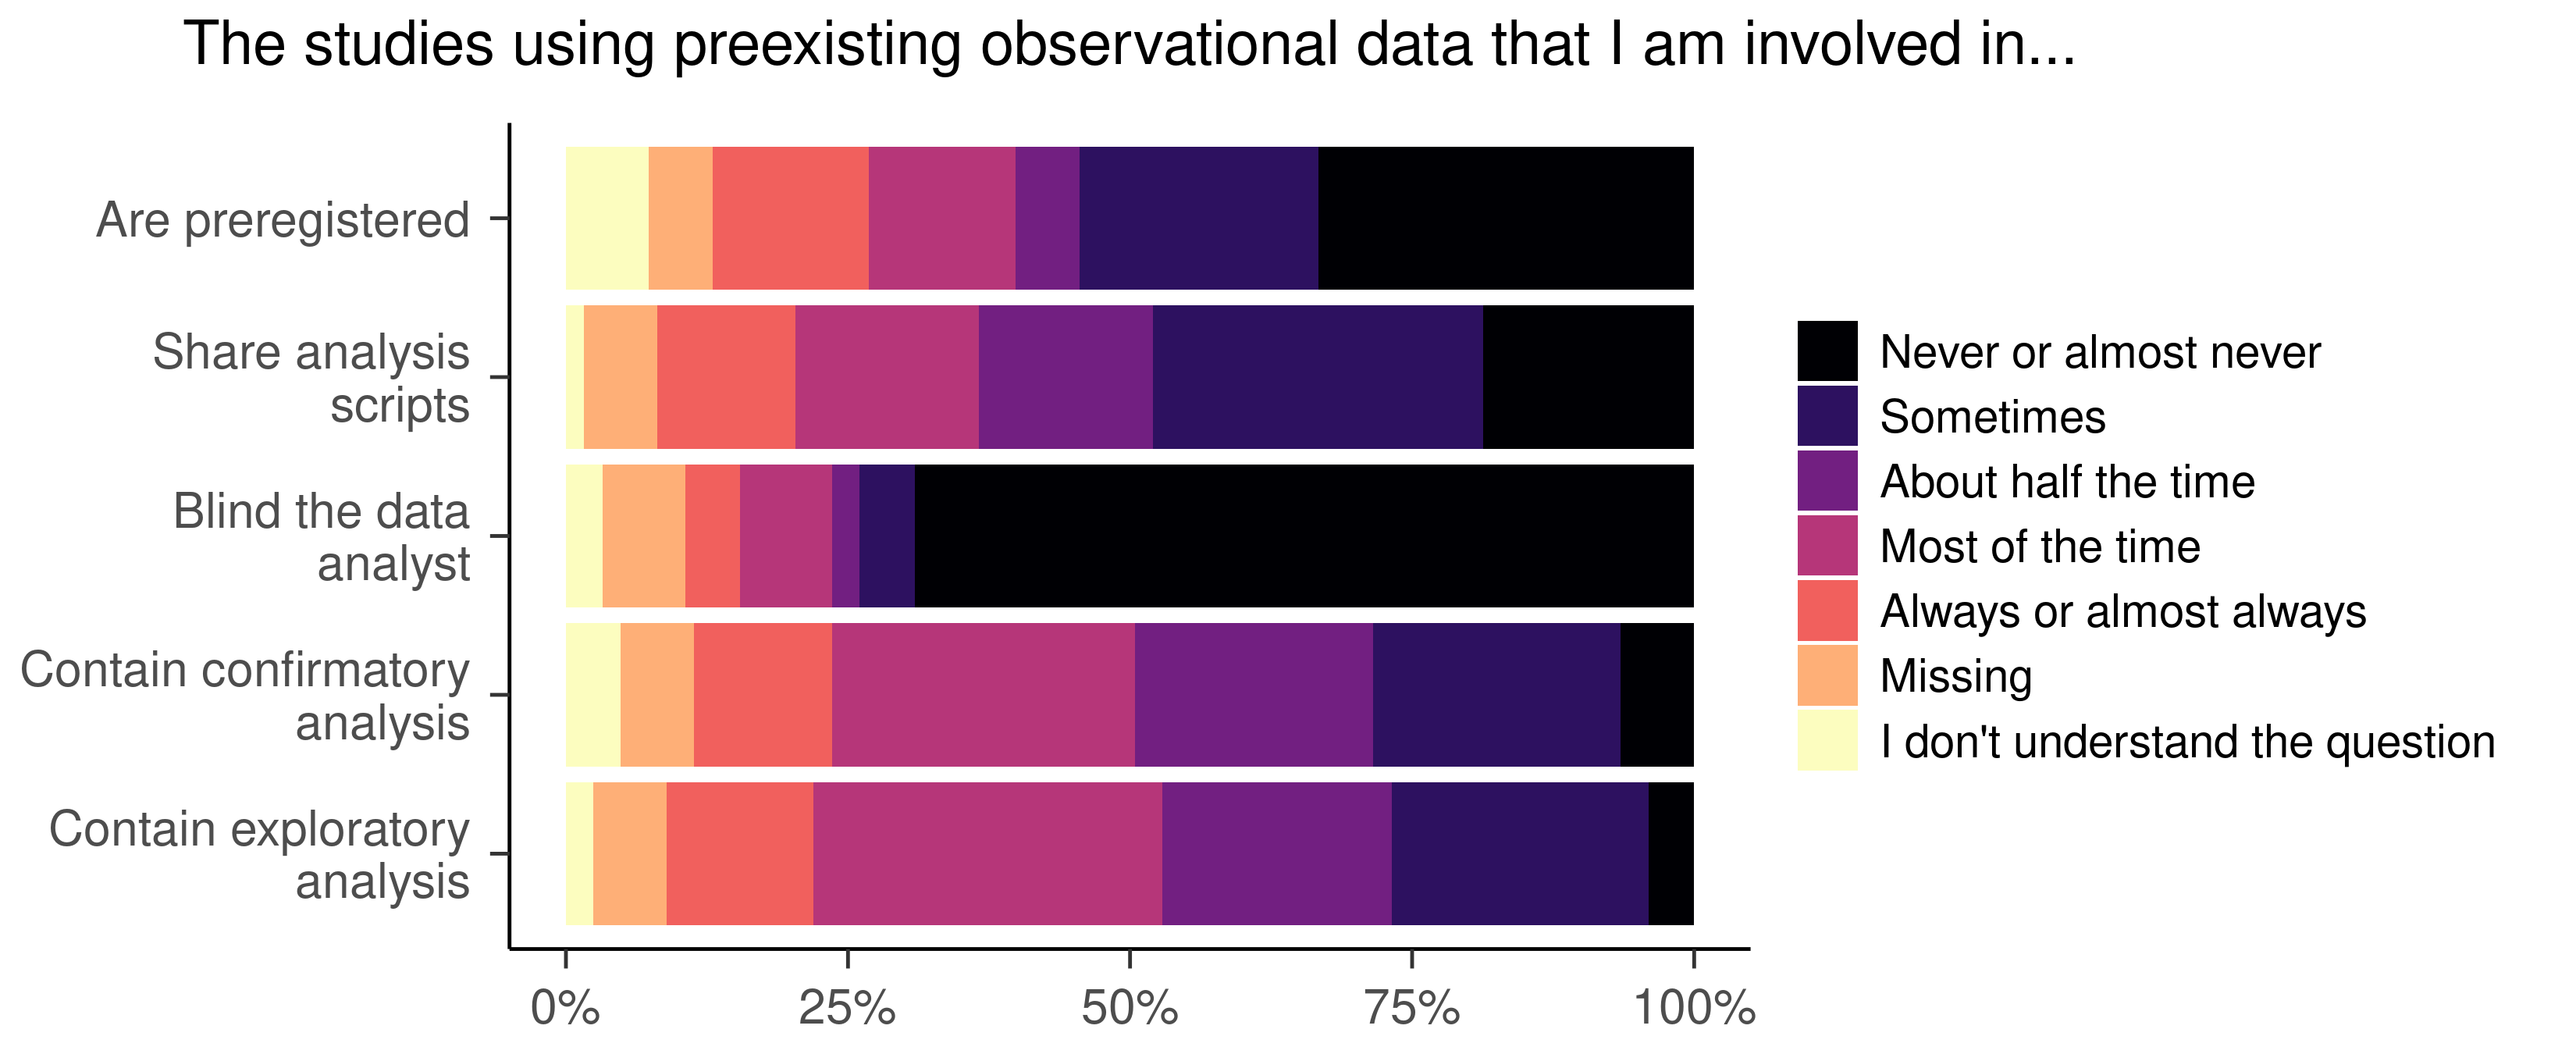
\includegraphics[width=1\linewidth]{figs/methodPlotAll-1} 

}

\caption{\textbf{Figure 2D. Responses to survey questions about the research practices of participants.}}\label{fig:methodPlotAll}
\end{figure}

{\smaller[1]
\begin{singlespace}



\end{singlespace}
}

25\% (26/106) of respondents agreed (versus 44\%; 47/106 who disagreed) that they would be less willing to use ALSPAC data if they were required to use an ECAW (Figure 3D). 51\% (50/98) agreed (21\%; 21/98 disagreed) that they would opt-in if ALSPAC ran a study on ECAWs. 54\% (54/100) agreed (11\%; 11/100 disagreed) that ALSPAC should run a study on ECAWs. 45\% (45/100) agreed (22\%; 22/100 disagreed) that they would prefer using an ECAW than using typical preregistration.

\begin{figure}[H]

{\centering 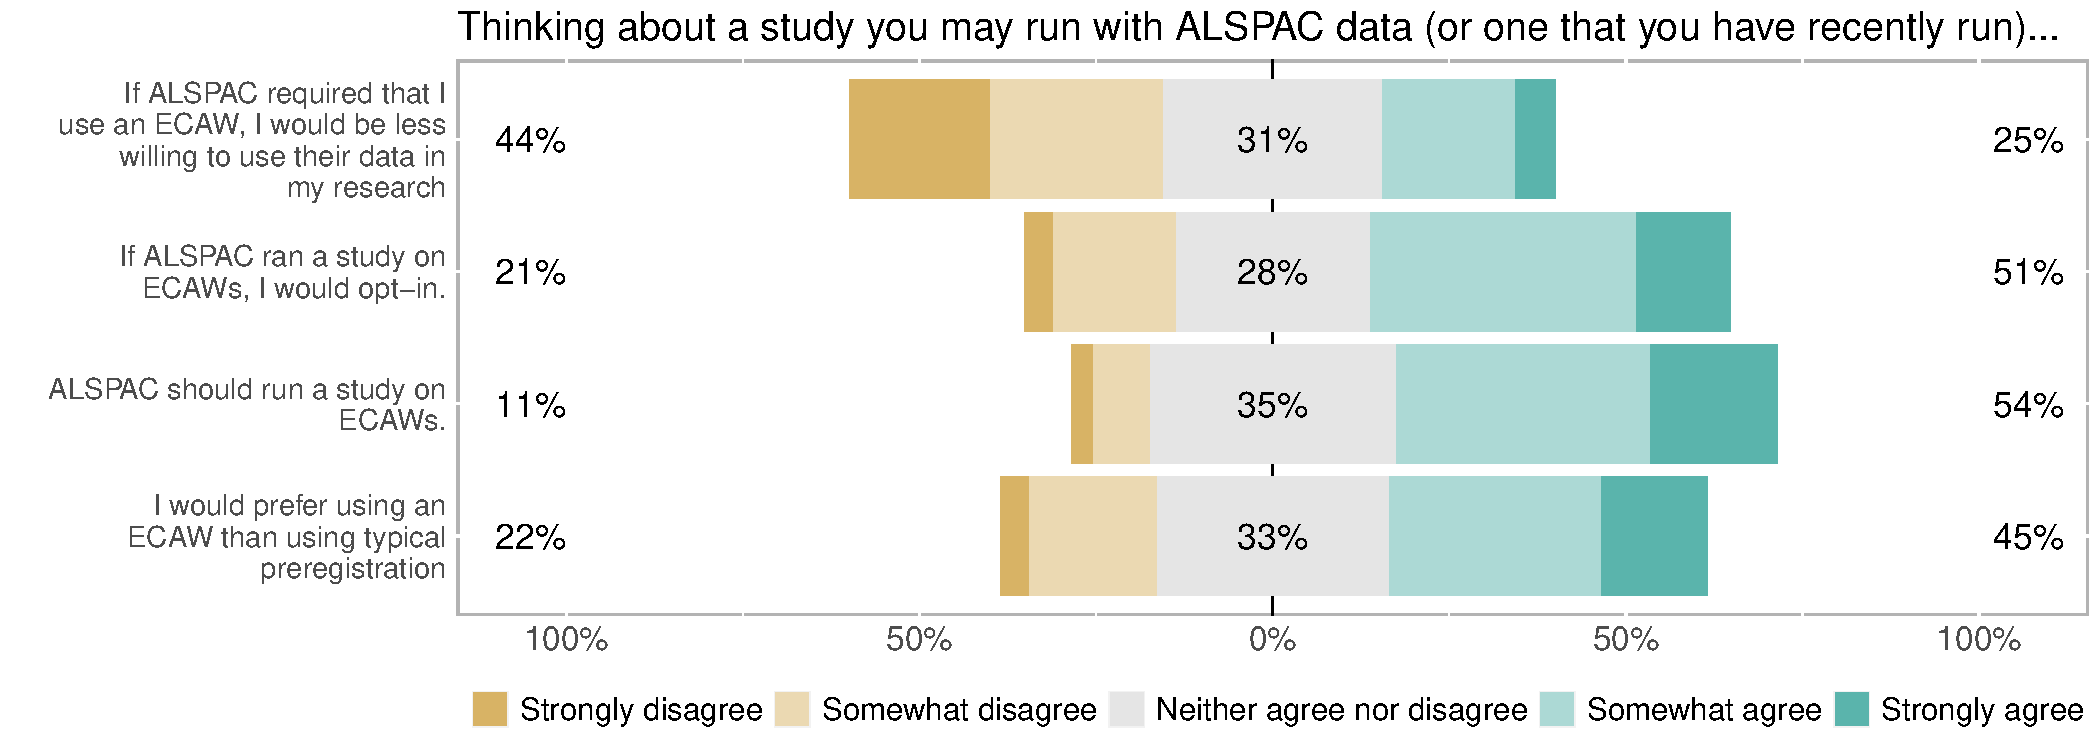
\includegraphics[width=1\linewidth]{figs/alspacPlotAll-1} 

}

\caption{\textbf{Figure 3D. Responses to survey questions about using ECAWs.} These bar charts exclude missing values (\emph{n} = 14; 14; 14; 14; respectively from top to bottom), responses of \emph{``I don't understand the question''} (\emph{n} = 0; 5; 2; 1), and responses of \emph{``Unsure''} (\emph{n} = 3; 6; 7; 8). Agreement with the first question may be slightly inflated due to the format of the questions in this block. Respondents with a highly positive inclination towards ECAWs would be expected to disagree with the first question, but agree with the next three questions. Four respondents agreed with all four statements, suggesting they may have glazed over the word ``less'' in the first question \protect\footnotemark[2]. Interpreting responses to the second and third question come with a degree of ambiguity as the survey did not specify what was meant by the term ``study'' \protect\footnotemark[3].}\label{fig:alspacPlotAll}
\end{figure}

{\smaller[1]
\begin{singlespace}



\end{singlespace}
}

\protect\footnotetext[2]{Another four respondents agreed with at least the first and second question, which appear contradictory. We did not preregister these considerations. More careful wording of these questions could have circumvented the ambiguity in interpreting these seemingly contradictory responses.}
\protect\footnotetext[3]{We intended for these questions to ask about ALSPAC running a trial on ECAWs. However, due to the ambiguity around the terms “study”, some respondents may have interpreted this as a survey, focus group, feasibility, or pilot type of study.}


\end{document}
